%%%%%%%%%%%%%%%%%%%%%%%%%%%%%%%%%%%%%%%%%
% Machine Learning @ PUC-Rio 2017.2
%%%%%%%%%%%%%%%%%%%%%%%%%%%%%%%%%%%%%%%%%
% Ian Albuquerque Raymundo da Silva - 1310451
% Clara de Mattos Szwarcman - 1310351
%%%%%%%%%%%%%%%%%%%%%%%%%%%%%%%%%%%%%%%%%

%%%%%%%%%%%%%%%%%%%%%%%%%%%%%%%%%%%%%%%%%
% Journal Article
% LaTeX Template
% Version 1.4 (15/5/16)
%
% This template has been downloaded from:
% http://www.LaTeXTemplates.com
%
% Original author:
% Frits Wenneker (http://www.howtotex.com) with extensive modifications by
% Vel (vel@LaTeXTemplates.com)
%
% License:
% CC BY-NC-SA 3.0 (http://creativecommons.org/licenses/by-nc-sa/3.0/)
%
%%%%%%%%%%%%%%%%%%%%%%%%%%%%%%%%%%%%%%%%%

%----------------------------------------------------------------------------------------
%	PACKAGES AND OTHER DOCUMENT CONFIGURATIONS
%----------------------------------------------------------------------------------------

\documentclass[twoside,twocolumn]{article}

\usepackage{blindtext} % Package to generate dummy text throughout this template 
\usepackage[utf8]{inputenc}
\usepackage{graphicx}

\usepackage[sc]{mathpazo} % Use the Palatino font
\usepackage[T1]{fontenc} % Use 8-bit encoding that has 256 glyphs
\linespread{1.05} % Line spacing - Palatino needs more space between lines
\usepackage{microtype} % Slightly tweak font spacing for aesthetics

\usepackage[english]{babel} % Language hyphenation and typographical rules

\usepackage[hmarginratio=1:1,top=32mm,columnsep=20pt]{geometry} % Document margins
\usepackage[hang, small,labelfont=bf,up,textfont=it,up]{caption} % Custom captions under/above floats in tables or figures
\usepackage{booktabs} % Horizontal rules in tables

\usepackage{lettrine} % The lettrine is the first enlarged letter at the beginning of the text

\usepackage{enumitem} % Customized lists
\setlist[itemize]{noitemsep} % Make itemize lists more compact

\usepackage{abstract} % Allows abstract customization
\renewcommand{\abstractnamefont}{\normalfont\bfseries} % Set the "Abstract" text to bold
\renewcommand{\abstracttextfont}{\normalfont\small\itshape} % Set the abstract itself to small italic text

\usepackage{titlesec} % Allows customization of titles
\renewcommand\thesection{\Roman{section}} % Roman numerals for the sections
\renewcommand\thesubsection{\roman{subsection}} % roman numerals for subsections
\titleformat{\section}[block]{\large\scshape\centering}{\thesection.}{1em}{} % Change the look of the section titles
\titleformat{\subsection}[block]{\large}{\thesubsection.}{1em}{} % Change the look of the section titles

\usepackage{fancyhdr} % Headers and footers
\pagestyle{fancy} % All pages have headers and footers
\fancyhead{} % Blank out the default header
\fancyfoot{} % Blank out the default footer
\fancyhead[C]{Supervised Learning with Fashion MNIST $\bullet$ December 2017 $\bullet$ Machine Learning @ PUC-Rio} % Custom header text
\fancyfoot[RO,LE]{\thepage} % Custom footer text

\usepackage{titling} % Customizing the title section

\usepackage{hyperref} % For hyperlinks in the PDF

%----------------------------------------------------------------------------------------
%	TITLE SECTION
%----------------------------------------------------------------------------------------

\setlength{\droptitle}{-4\baselineskip} % Move the title up

\pretitle{\begin{center}\Huge\bfseries} % Article title formatting
\posttitle{\end{center}} % Article title closing formatting
\title{Supervised Learning with Fashion MNIST} % Article title
\author{%
\textsc{Clara de Mattos Szwarcman}\thanks{Clara's student ID: 1310351} \\[1ex] % Your name
\normalsize Pontifícia Universidade Católica do Rio de Janeiro \\ % Your institution
\normalsize \href{mailto:clara_szw@hotmail.com}{clara\_szw@hotmail.com} % Your email address
\and % Uncomment if 2 authors are required, duplicate these 4 lines if more
\textsc{Ian Albuquerque Raymundo da Silva}\thanks{Ian's student ID: 1310451} \\[1ex] % Second author's name
\normalsize Pontifícia Universidade Católica do Rio de Janeiro \\ % Second author's institution
\normalsize \href{mailto:ian.albuquerque.silva@gmail.com}{ian.albuquerque.silva@gmail.com} % Second author's email address
}
\date{\today} % Leave empty to omit a date
\renewcommand{\maketitlehookd}{%

}

%----------------------------------------------------------------------------------------

\begin{document}

% Print the title
\maketitle

%----------------------------------------------------------------------------------------
%	ARTICLE CONTENTS
%----------------------------------------------------------------------------------------

\section{Introduction}

\lettrine[nindent=0em,lines=3]{T} he MNIST dataset is considered the "hello world" of Machine Learning.
Current results achieve over 99.7\% accuracy using different techniques
\cite{LWan:2013dg} \cite{DCirean:2012dg} \cite{ISato:2015dg} \cite{JRChang:2015dg} \cite{CYLee:2015dg}.
Also, many good techniques do not work well on this dataset because of its simplicity \cite{CFran:2017dg}.
With that in mind, the Fashion MNIST dataset \cite{FashionMNIST} was created. It has same size and format
of the MNIST dataset meaning that
it should be as simple to use, but its images consist of fashion items which are supposedly harder to
classify.

The goal of this work is to explore different techniques of supervised learning for classifying the images
in the Fashion MNIST dataset. We want to measure the accuracy of our tests and compare them with different
results on the same dataset, while also trying to obtain some intuition behind the data.\


\section{DataSet}

	The Fashion MNIST dataset is composed by 70.000 grayscale(0-255) images of size 28x28 labeled into the following 10 different classes: T-shirt/top, Trouser, Pullover, Dress, Coat, Sandal, Shirt, Sneaker, Bag and Ankle boot.\ref{fig:fashionex} is an example of one of the images in the dataset.
	
	\begin{figure}[h]
    \begin{center}
        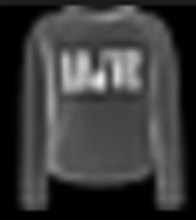
\includegraphics[scale=0.8]{fashionExample.png}
        \caption{Image Example\label{fig:fashionex}}
    \end{center}
    \end{figure}
    
    For the implementation we used Python and sklearn\cite{scikitlearn} and tensorflow \cite{tensorflow} libraries. The input for the algorithms are the pixels values.
	

%----------------------------------------------------------------------------------------

\section{Preparation}

The Fashion MNIST is already subdivided into two sets. A set of 60.000 images (the training set)
and a set of 10.000 images (the test set). The idea is to learn with the training set and then
evaluate the performance of our trained model with the test set.

We will be using the standard accuracy as a metric for our tests:
\begin{equation}
\label{eq:acc}
accuracy = \frac{\#(correct\_classifications)}{\#(test\_set\_size)}
\end{equation}

The dataset is already provided as a list of (28*28)+1 sized vectors corresponding
to each of the 28*28 pixels of the image plus 1 entry for the classification.
Since each pixel value was an integer from 0 to 255, we have opted to divide
each value by 255 to achieve features that goes from 0 to 1.

%----------------------------------------------------------------------------------------

\section{Known Results}

The Fashion MNIST repository contains some benchmarks using the python library
scikit-learn \cite{scikitlearnbenchmark}. They are not meant
to be efficient or good, but they work as a baseline for our project.
The best result (corresponding to the best selection of parameters tested)
of each algorithm are displayed in table \ref{table:scikit-benchmark}.

\begin{table}
\centering
\begin{tabular}{llr}
\toprule
Algorithm Name & Best Accuracy (\%) \\
\midrule
SVC & $89.7$ \\
Gradient Boosting & $88.8$ \\
Random Forest & $87.9$ \\
MLP & $87.7$ \\
K-Neighbors & $86.0$ \\
Logistic Regression & $84.0$ \\
SGD & $82.9$ \\
Decision Tree & $80.1$ \\
\bottomrule
\end{tabular}
\caption{Fashion MNIST Scikit-Learn Benchmark \cite{scikitlearnbenchmark} }
\label{table:scikit-benchmark}
\end{table}

The current state of art for the Fashion MNIST dataset is a recent one, with 96.3\% accuracy using Wide
Residual Networks using random erasing data augmentation \cite{randomerasingdataaugmentationpaper}.
We will consider this as the ceiling accuracy for our project.

%------------------------------------------------

\section{Approaches}

\subsection{Random Classifier}

To test our framework, we implemented a random classifier that simply guesses one of the 10 classes. The accuracy was 10\% as expected.

\subsection{K-Nearest-Neighbors (KNN)}

\subsubsection{Own implementation}

Our first attempt at the problem was implementing the K-Nearest-Neighbors algorithm ourselves.
We tried using the Euclidean distance as the metric and K = 50 as the parameters for the algorithm.
For that, we obtained an accuracy of 75.80\%, quite far from the scikit-learn benchmark.

This algorithm was pretty fast to implement.
Since its training consists in only saving the training set, it is pretty fast.
However, it does take a lot of time to classify each example.

\subsubsection{Distance from Mean}

Inspired by the KNN algorithm, we implemented a "distance from mean" algorithm in which for the training we
take the mean of each group of instances of the same class and for the testing we simply classify as the nearest
of the 10 means obtained in the training part.

This is basically a worse version of the KNN and the results were worse accordingly.
We obtained an accuracy of 67.68\%.
The benefits were the fact that it was easy to implement, fast to train and fast to classify.

\subsubsection{Scikit-Learn Implementation}

We also tested for the Scikit-Learn implementation for the KNN algorithm.
This time, we tested for K = 5 neighbors using the Manhattan distance.
Our obtained accuracy was 86.23\%, the exact accuracy from the benchmark, as expected.

\subsubsection{Scikit-Learn w/ Haar Transform Pre-Processing}

For the next test, we tried to pre-process the dataset by changing the feature space. We  maintained the parameters K = 5 and
Manhattan distance, but also used the Haar transform to change the feature space. The idea was to use features that described the frequencies
in the image, allowing a more global description of the image. However, it did not achieve good results, resulting in an accuracy of 84.0\%, lower than
the algorithm without the Haar Transform pre-processing.

\subsection{Single Layer Perceptron}

\subsubsection{Standard Implementation}

We implemented ourselves a single layer perceptron and trained it with only 1 iteration over the dataset.
We did not invest a lot of effort in this approach because it relies on the assumption that the dataset
is linearly separable for the algorithm to converge, which clearly is not the case for the dataset.
We obtained an accuracy of 75.8\% for this approach

\subsubsection{MIRA (Margin-infused relaxed algorithm)}

We made some changes to the update step of the algorithm so it took into account how much
each error should affect the weights of the perceptron, using the Margin-infused relaxed algorithm
technique. We obtained slightly better result, with an accuracy of 76.99\%.

\subsection{SVM (Scikit-Learn Implementation)}

\subsubsection{Polynomial Kernel}

For the SVM we used the Scikit-Learn implementation. We first tested with a 3rd degree polynomial kernel and with a penalty parameter C = 10, since
it was the parameters used for the benchmark. We obtained an accuracy of 87.23\%, which is slightly different from the accuracy described in the benchmark (87,23\%).

\subsubsection{Polynomial Kernel w/ Pre-Processing}

We tried to improve the results by pre-processing the dataset by downscaling the images to 7x7, normalizing the dataset by feature (pixel) and also adding
to the algorithm input rotations of the original dataset from -10 to 10 degrees, varying degree by degree.
With that technique, we obtained an accuracy of 84.91\%, which was worse than without the pre-processing. We suspect that down sampling the dataset
to 7x7 images caused too much information loss.

Because of that, we changed the down sampling to 14x14 and also changed the rotation interval to the interval -5 to 5 degrees.
The new accuracy was 89.39\%, an improvement of about 2\% compared to the example without the pre-processing.

It is also important to note that the pre-processing heavily improved the accuracy of the algorithm when using a small subset of the
original dataset. For instance, for 100 instances, the accuracy was improved from 43.69\% to 64.21\% and for 1000 instances it was
improved from 59.10\% to 78.56\%. It is probably due to the fact that adding the rotation benefits a lot small datasets that do not contain
enough data for the generalization necessary for good results.

\subsubsection{Gaussian Kernel}

We also tested for a gaussian kernel, with parameter C = $10^6$ and gamma = $4 10^-7$ since it achieved good results from previous works.
As expected, we obtained better accuracy, achieving 90.13\% for those parameters.

\subsubsection{Gaussian Kernel w/ Rotations and Canny Filterl}

By adding rotations from -5 to 5 degrees, without down sampling, and also applying the canny filter (an edge detection filter)
for the dataset, we achieved a result of 80.36\%. Even though we thought that applying the canny filter was a good idea to improve
the significance features of the image, it clearly was not the case.

\subsection{Convolutional Neural Networks}

     The Convolutional Neural Networks (CNNs) are the current state-of-the-art for the Fashion-MNIST dataset with 96.3\% accuracy \cite{randomerasingdataaugmentationpaper}. For all tests with CNNs the values of the pixels were divided by 255, so that the values are always between 0 and 1. The first CNN that we used was based on the 1994s LeNet5 \cite{yannLeCun:1998}, one of the first CNNs, that has a 99.05\% accuracy for the MNIST dataset \cite{yannLeCun:mnist}. We used the same layers and kernel sizes but with more features on each convolutional layer. \ref{fig:lenet5} shows the architecture used for the first CNN test.

    \begin{figure}[h]
    \begin{center}
        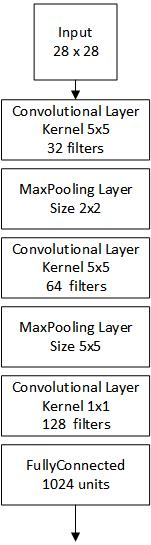
\includegraphics[scale=0.8]{lenet5Arch.jpg}
        \caption{LeNet5 based Architecture\label{fig:lenet5}}
    \end{center}
    \end{figure}
    
    
    We trained the network for 200 epochs and got an accuracy of 89.02\%, then, to increase the examples in the training set, we added rotations from -5 to 5 degrees and got 89.81\%.
    
    Seeking to improve our accuracy, we used a more complex and deeper CNN as base, the Very Deep Convolutional Networks \cite{DBLP:journals/corr/SimonyanZ14a} used in the  ImageNet Challenge. Since this is a deep CNN and made for 224x224 RGB images, we adapted to a smaller network with a receptive field of 28x28 and fewer units on the fully connected layer. \ref{fig:vgg} shows the architecture of the new CNN.
    
    \begin{figure}[h]
    \begin{center}
        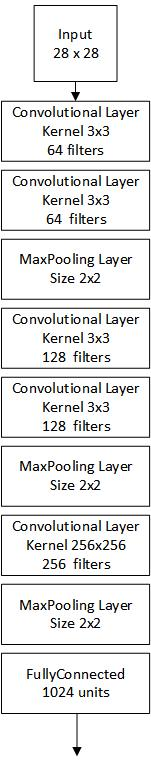
\includegraphics[scale=0.65]{vggArch.jpg}
        \caption{VGG based Architecture\label{fig:vgg}}
    \end{center}
    \end{figure}
    
    The accuracy obtained from training the new network for 300 epochs was 90.06\%, and for 938 epochs, 91.27\%. When we tried to increase the number of epochs again, the accuracy dropped slightly, so we went to another approach. \ref{fig:lossRateVGG} shows the value of the loss rate given the number of steps.
    
    
    \begin{figure}[h]
    \begin{center}
		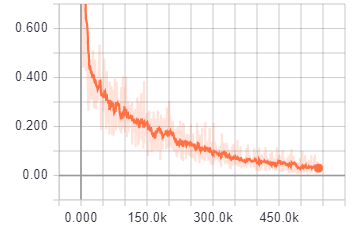
\includegraphics[scale=0.6]{lossRateVGG.png}
        \caption{Loss Rate for VGG based network\label{fig:lossRateVGG}}    
    \end{center}
    \end{figure}
    
    Our next approach was to use Random Erasing as data augmentation, since it was used in the state-of-the-art implementation. Random Erasing randomly
selects a rectangle region in an image and erases its pixels with random values, which reduces the risk of over-fitting. For 300 epochs the accuracy was . Seeing that adding only the Random Erasing technique decreased the accuracy, we combined it with the rotation from -5 to 5 degrees.
    
    

%----------------------------------------------------------------------------------------
%	REFERENCE LIST
%----------------------------------------------------------------------------------------

\bibliography{references}
\bibliographystyle{plain}

%----------------------------------------------------------------------------------------

\end{document}
